\section{Multipoles}

\subsection{Spherical Multiple Moment}\label{Spherical Multiple Moment}

\textbf{1):}

The first thing one should do is to sketch how the system looks like:

\begin{figure}[h]
	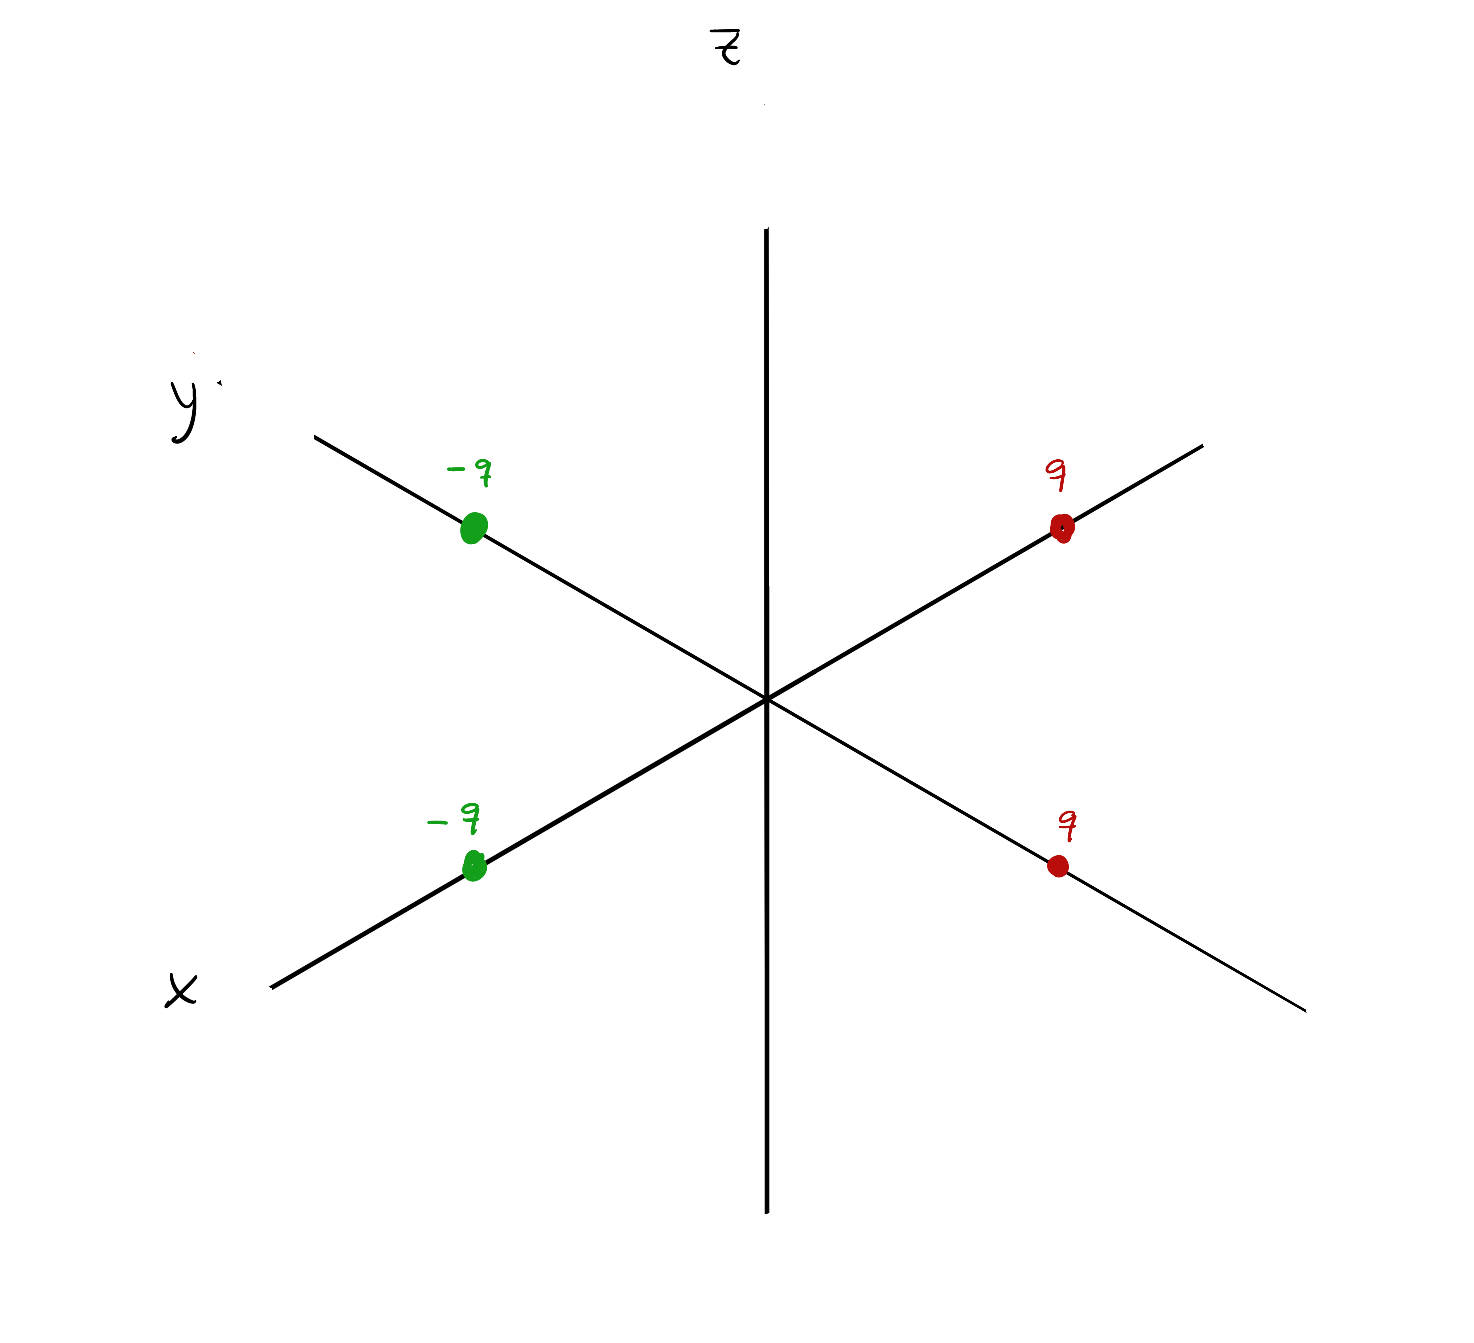
\includegraphics[width=7cm]{figures/Quadrupole.png}
	\centering
	\caption{The distribution of the charges.}
\end{figure}

Given this charge distribution, we already know that the total charge of the system is $Q=0$. Let's first prove that the charge distribution integrated over the whole space yields also a zero. We also know that the total charge is:
	
\begin{equation}
	Q_{T} = \int \rho (\vec{x}') d^{3}x' = \int \rho(r', \theta', \phi')\: r'^{2} \sin\theta' dr' \: d\phi' \: d\theta'.
\end{equation}

Recall that $\delta$ changes between Cartesian and spherical coordinates as:

\begin{equation}
	\delta (\vec{x}' - \vec{x}) \rightarrow \tfrac{1}{r'^{2} \sin \phi'} \delta (r' -r) \delta(\theta' -\theta) \delta (\phi' - \phi).
\end{equation}

So the charge density for the four point charged particles is:

\begin{equation}
	\begin{split}
		\rho (r') = \tfrac{q}{r'^{2} \sin\phi'} (\delta (r' -a) &\delta(\theta' - 0) \delta (\phi' - \tfrac{\pi}{2}) + \delta (r' -a) \delta(\theta' - \tfrac{\pi}{2}) \delta (\phi' - \tfrac{\pi}{2})-\\
		\delta (r' -a) &\delta(\theta' - \pi) \delta (\phi' - \tfrac{\pi}{2}) -\delta (r' -a) \delta(\theta' - \tfrac{3\pi}{2}) \delta (\phi' - \tfrac{\pi}{2})).
	\end{split}
\end{equation}

Which integrated over the whole space $r \:\epsilon\: [0, \infty],\: \theta\: \epsilon \:[0, 2\pi], \:\phi \:\epsilon [0, \pi]$ yields a total charge $Q_{T}=0$ as expected. What about the quadrupoles?

\textbf{2):}

They also want us to calculate the multiple moments (recall: The charge density $\times$ the harmonics). This is given by the following formula as:

\begin{equation}
	\begin{split}
	q_{lm} &= \int Y^{*}_{lm} (\theta', \phi')r'^{l} \rho (\vec{x}') d^{3}x'=\\
	&= \int Y^{*}_{lm}r'^{l} \tfrac{q \:\delta (r' -a) \delta (\phi' - \tfrac{\pi}{2})}{r'^{2} \sin \phi}\: \left( \delta(\theta' - 0) + \delta(\theta' - \tfrac{\pi}{2}) -\delta(\theta' - \pi) - \delta(\theta' - \tfrac{3\pi}{2})\right)\: r'^{2} \sin \phi \: d^{3}x'=\\
	& = q \: a^{l} \left( Y^{*}_{lm} (0, \tfrac{\pi}{2}) + Y^{*}_{lm} (\tfrac{\pi}{2}, \tfrac{\pi}{2}) - Y^{*}_{lm} (\pi, \tfrac{\pi}{2}) - Y^{*}_{lm} (\tfrac{3\pi}{2}, \tfrac{\pi}{2})\right).
	\end{split}
\end{equation}

This can be further simplified, simply using the definition of spherical harmonics given by:

\begin{equation}
	Y_{lm} (\theta, \phi) = \sqrt{\tfrac{2l+1}{4\pi}\tfrac{(l-m)!}{(l+m)!}} P^{m}_{l} (\cos \phi) e^{im\theta}, \quad \quad P^{m}_{l} (x) = (-1)^{m} (1- x^{2})^{m/2} \tfrac{d^{m}}{dx^{m}} P_{l} (x).
\end{equation}

So a more specific expression for $q_{lm}$ is:

\begin{equation}
	q_{lm} = q \: a^{l} \: \sqrt{\tfrac{2l+1}{4\pi}\tfrac{(l-m)!}{(l+m)!}} P^{m}_{l} (\cos \tfrac{\pi}{2}) \left(1 + (-i)^{m} - (-1)^{m}- i^{m}\right)
\end{equation}

From here, one just have to compute the first non-zero entries. It follows that:

\begin{equation}
	q_{0,0} = q_{1,0} = q_{0,1} = 0, \quad \quad q_{1,1} = a \: \sqrt{\tfrac{3}{2\pi}}(1-i), \quad q_{1,-1} = -a \: \sqrt{\tfrac{3}{2\pi}}(1+i).
\end{equation}

\subsection{Multiple Moments in Cartesian Coordinates}\label{Multiple Moments in Cartesian Coordinates}
\textbf{\textcolor{red}{UNDER CONSTRUCTION}}


\subsection{Exterior Multipoles for a Specified Potential on a Sphere}\label{Exterior Multipoles for a Specified Potential on a Sphere}


\textbf{1):}

The general form of a spherical multipole expansion is given by:

\begin{equation}\label{initialpotential}
	\Phi(r,\theta, \phi)=\sum_{\ell=0}^{\infty} \sum_{m=-\ell}^{\ell}\left( A_{\ell m} r^{\ell}  + \frac{B_{\ell m}}{r^{\ell+1}} \right) Y_{\ell m}(\Omega).
\end{equation}

As we are asked to show the general form of an \textbf{exterior} multipole expansion, we have to get rid of $A_{\ell m}$ as this coefficient is only for $r< R$ cases. For $B_{\ell m}$ we have the basic description:

\begin{equation}
	B_{\ell m}=\frac{4 \pi}{2 \ell+1} \int \rho\left(\mathrm{r}^{\prime}\right) r^{\prime \ell} Y_{\ell m}^{\star}\left(\Omega^{\prime}\right) d V^{\prime}.
\end{equation}

As we have to express eq(\ref{initialpotential}) without the $B$ coefficient, we need to find its explicit value for $\forall r> R$. Here we can abuse from spherical harmonic properties as:
	
\begin{equation}
	\begin{split}
		\Phi(R, \Omega)&=\sum_{\ell=0}^{\infty} \sum_{m=-\ell}^{\ell} A_{\ell m} \frac{Y_{\ell m}(\Omega)}{R^{\ell+1}}= \\
		&= 	\text{Multiply both sides times $Y^{\star}_{\ell' m'}$}\rightarrow \\
		\int \Phi\left(R, \Omega^{\prime}\right) Y_{\ell^{\prime} m^{\prime}}^{\star}\left(\Omega^{\prime}\right) d \Omega^{\prime}&=\sum_{\ell=0}^{\infty} \sum_{m=-\ell}^{\ell} \frac{B_{\ell m}}{R^{\ell+1}} \int Y_{\ell m}\left(\Omega^{\prime}\right) Y_{\ell^{\prime} m^{\prime}}^{\star}\left(\Omega^{\prime}\right) d \Omega^{\prime} .
	\end{split}
\end{equation}

The orthonormality of the spherical harmonics gives the expansion coefficients as:

\begin{equation}
	\begin{split}
		\int d\Omega Y^{\star}_{\ell',m'} Y_{\ell m} &= \delta_{\ell' \ell} \: \delta_{m' m} \rightarrow \\
		B_{\ell m}&=R^{\ell+1} \int \Phi\left(R, \Omega^{\prime}\right) Y_{\ell^{\prime} m^{\prime}}^{\star}\left(\Omega^{\prime}\right) d \Omega^{\prime}.
	\end{split}
\end{equation}

Then, all together looks like:

\begin{equation}
	\Phi(\mathrm{r})=\sum_{\ell=0}^{\infty} \sum_{m=-\ell}^{\ell}\left(\frac{R}{r}\right)^{\ell+1} Y_{\ell m}(\Omega) \int \varphi\left(R, \Omega^{\prime}\right) Y_{\ell^{\prime} m^{\prime}}^{\star}\left(\Omega^{\prime}\right) d \Omega^{\prime}, \quad r>R.
\end{equation}
	
\textbf{2):}

We need to solve how the potential $\Phi$ looks like in asymptotic limit ($r\rightarrow \infty$) for the given distribution. In order to craft this, we have to find a linear combination of harmonics that can reproduce the behaviour of the combination of the octants. This can be done by brute force, integrating each of the different 8 regions for given solid angle or to think a little bit to reduce the required computation.

We can see that $V$ changes to $\pm$ every $\pi/2$ in $\phi$ angle. We know that the associated number in the harmonics to this angle is $m$. Checking the values of $Y_{\ell m}$, we see that the change will occur when $m = \pm 2$, because:
	
\begin{equation}
	Y_{\ell \pm 2} \propto e^{\pm 2 i \phi} \rightarrow e^{\pm i \pi} = \pm 1.
\end{equation}

So, if $|m| =2$, $\ell \ge 2$. We find a minimum value for $\ell$. What about 2? Then, the associated spherical harmonic value reads:
	
\begin{equation}
	Y_{2 2} \propto \sin^{2} \theta e^{2 i \phi}.
\end{equation}

This cannot be,as we want the associated value of $\theta$ to vary as $\pm$ when moving around the octants. But if we check the following harmonic:
	
\begin{equation}
	Y_{3 \pm 2} = \tfrac{1}{4\pi} \sqrt{\tfrac{105}{2\pi}} \sin^{2}\theta \cos \theta e^{\pm 2 i \phi}. 
\end{equation}

Where $\cos$ will allow that variation. Then $\Phi = \text{L.C} \left(Y_{3, \pm2}\right)$. We are close to be able to offer an expression for the potential when $r \rightarrow \infty$. Recall also that $\Phi|_{r=R} = \pm V$ and when $r\rightarrow \infty$, only the smallest allowed value of $\ell$ will contribute in the leading order of the expression. With all this, we can state that: 
	
\begin{equation}
	\Phi(\mathrm{r})=V\left(\frac{R}{r}\right)^{4} 2 \sqrt{\frac{2 \pi}{105}}\left(Y_{32}+Y_{3-2}\right)=V\left(\frac{R}{r}\right)^{4} \sin ^{2} \theta \cos \theta \cos 2 \phi, \quad r \rightarrow \infty.
\end{equation}


\subsection{Radiating Fidget Spinner}\label{Radiating Fidget Spinner}

So we want to study this system and get its values of $\mathbf{p}, \mathbf{m}$ and $Q_{ij}$. Let the distance from the axis of rotation to the charges be $R$, as displayed in the following sketch:

\begin{figure}[h]
	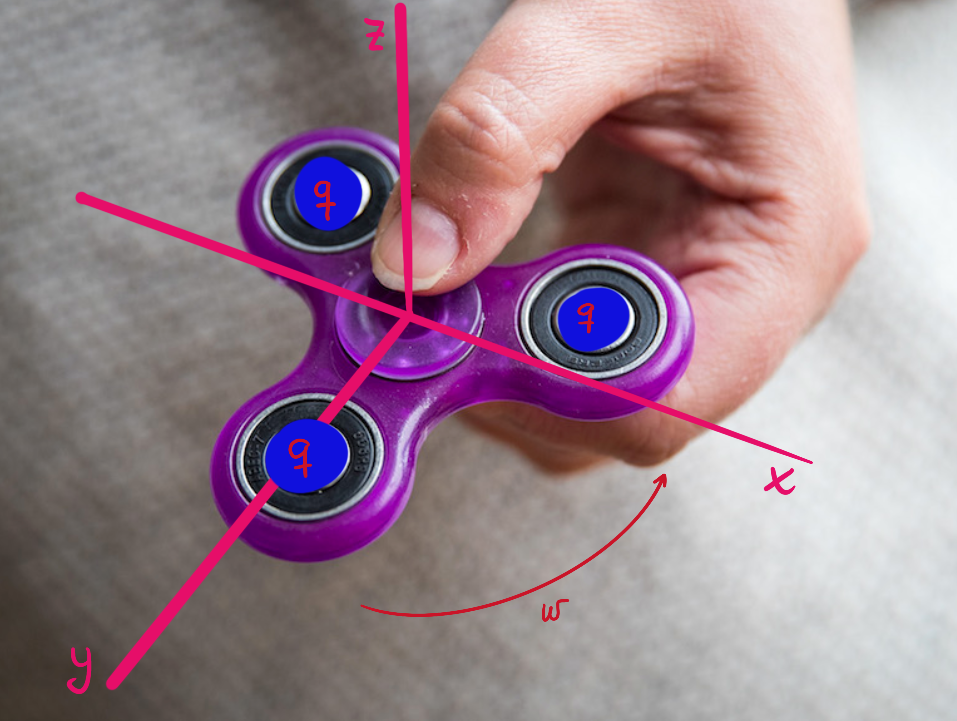
\includegraphics[width=8cm]{figures/Fidgetspinners.png}
	\centering
	\caption{We can imagine we placed a charge in each of the inner holes.}
\end{figure}

The electric dipole moment, as we know, is given by:

\begin{equation}
	\mathbf{p}=\int d^{3} r \:\mathrm{r} \:\rho(\mathbf{r}, t).
\end{equation}

Hence, we need to write down the position of the charges in this spinning device. We know that each of them are at $2\pi/3$ angular distance, so:

\begin{equation}
	\begin{split}
		\mathbf{x}_{1} &= (R \cos \left(\omega t+0\right),R \sin \left(\omega t+0\right), 0),\\
		\mathbf{x}_{2} &= (R \cos \left(\omega t+\tfrac{2\pi}{3}\right),R \sin \left(\omega t+\tfrac{2\pi}{3}\right), 0),\\
		\mathbf{x}_{3} &= (R \cos \left(\omega t+\tfrac{4\pi}{3}\right),R \sin \left(\omega t+\tfrac{4\pi}{3}\right), 0).\\
	\end{split}
\end{equation}

We therefore have:

\begin{equation}
	p_{x}=q \sum_{i=1}^{3} x_{i}=R q(\cos (\omega t)+\cos (\omega t+2 \pi / 3)+\cos (\omega t-2 \pi / 3))=0
\end{equation}

and, similarly, $p_{y}= p_{z}=0$. So, there is no electric dipole radiation.

The current density is given by $\mathbf{j}(\mathbf{r}, t)=\mathbf{v} \rho(\mathbf{r}, t)$ where the velocity $\mathbf{v}$ points (locally) in the direction of the particle motion with magnitude $v=R \omega$. The magnetic dipole moment can be calculated as:

\begin{equation}
	\begin{split}
		\mathbf{m}= \int d^{3} r \:\mathbf{r} \times \mathbf{j}&=\int d^{3} r \underbrace{\mathbf{r} \times \mathbf{v}}_{(x,y,0)\times (x,y,0)= \hat{z}} \rho(\mathbf{r}, t)=\\
		&= R^{2} \omega \:\hat{\mathbf{z}} \int d^{3} r \rho(\mathbf{r}, t)=3 \omega q R^{2} \:\hat{\mathbf{z}} .
	\end{split}
\end{equation}

Observe that the magnetic dipole moment is time-independent! Therefore, there is no magnetic dipole radiation.

So far, no interesting properties for this system. What about the quadrupole momentum? The components of the electric quadrupole tensor are:

\begin{equation}
	Q_{i j}= \int d^{3} x \: \left(3 x^{i}x^{j} - r^{2} \delta^{ij}\right)\rho(\mathbf{x}, t).
\end{equation}

The symmetry of $\rho$ with respect to the $x$ -axis dictates that $Q_{x y}=0 $ (Compute it yourself to check that everything nicely cancels). Since the charges all lie in the plane $z=0$, we find that  $Q_{x z}=Q_{y z}=Q_{z z}=0$. So the only non-zero entries of $Q_{ij}$ are:

\begin{equation}
	\begin{split}
		Q_{x x} &=q \sum_{i=1}^{3} x_{i}^{2}=R^{2} q\left(\cos ^{2}(\omega t)+\cos ^{2}(\omega t+2 \pi / 3)+\cos ^{2}(\omega t-2 \pi / 3) -1 \right) =\\
		&=3 R^{2} q(\cos (2 \omega t)+\cos (2 \omega t-2 \pi / 3)+\cos (2 \omega t+2 \pi / 3))=\frac{3}{2} R^{2} q.
	\end{split}
\end{equation}

and, recall that $Tr (Q) =0$, so $Q_{y y}= - Q_{x x}=-\frac{3}{2} R^{2} q .$ Since $Q$ is time-independent, there is no electric quadrupole radiation either.